\chapter{Ejemplo práctico de aplicación}
\label{chap:ejemplo-practico-aplicacion}
Una vez explicado cómo funciona el paquete, se puede realizar una demostración práctica tomando como ejemplo los módulos fotovoltaicos que tiene en su azotea la Escuela Técnica Superior de Ingeniería y Diseño Industrial (en adelante la ETSIDI).

Se tomará de base un estudio realizado por profesores de la escuela \cite{adrada17}, en el cual comparan la producción energética de seis tipos de tecnologías fotovoltaicas.

En este ejemplo se realizará el mismo análisis tomando tres herramientas distintas: \texttt{solaR}, para poder tomar como referencia el paquete del que sale, apreciando las mejoras del programa. \texttt{PVSyst}, ya que es uno de los softwares más usados en el ámbito de la fotovoltaica y puede servir como punto de referencia. Y, por último, \texttt{solaR2}.

\section{\texttt{solaR}}
\label{sec:orgf0b76bb}
\label{sec:solaR}
Se empieza inicilizando el paquete:
\begin{lstlisting}[numbers=left,language=r,label= ,caption= ,captionpos=b]
library(solaR)
\end{lstlisting}

\begin{verbatim}
Cargando paquete requerido: zoo

Adjuntando el paquete: 'zoo'

The following objects are masked from 'package:base':

    as.Date, as.Date.numeric

Cargando paquete requerido: lattice
Cargando paquete requerido: latticeExtra
Time Zone set to UTC.
\end{verbatim}

En el estudio anterior, se recopilaron datos intradiarios de irradiación intradiaria. Sin embargo, estos datos fueron tomados en un plano inclinado, por lo que ni \texttt{solaR}, ni \texttt{solaR2} son capaces de interpretarlos correctamente. En su lugar, para este ejemplo se van a tomar datos horarios de la plataforma \texttt{PVGIS} \cite{pvgis} de los años 2013, 2014 y 2015 en la localización de la ETSIDI.
\begin{lstlisting}[numbers=left,language=r,label= ,caption= ,captionpos=b]
etsidi_1315 <- readBDi(file = 'TFG/data/PVGIS_1315.csv',
                       lat = 40.4, time.col = 'Dates',
                       format = '%Y-%m-%d %H:%M:%S')
xyplot(etsidi_1315)
\end{lstlisting}

\begin{center}
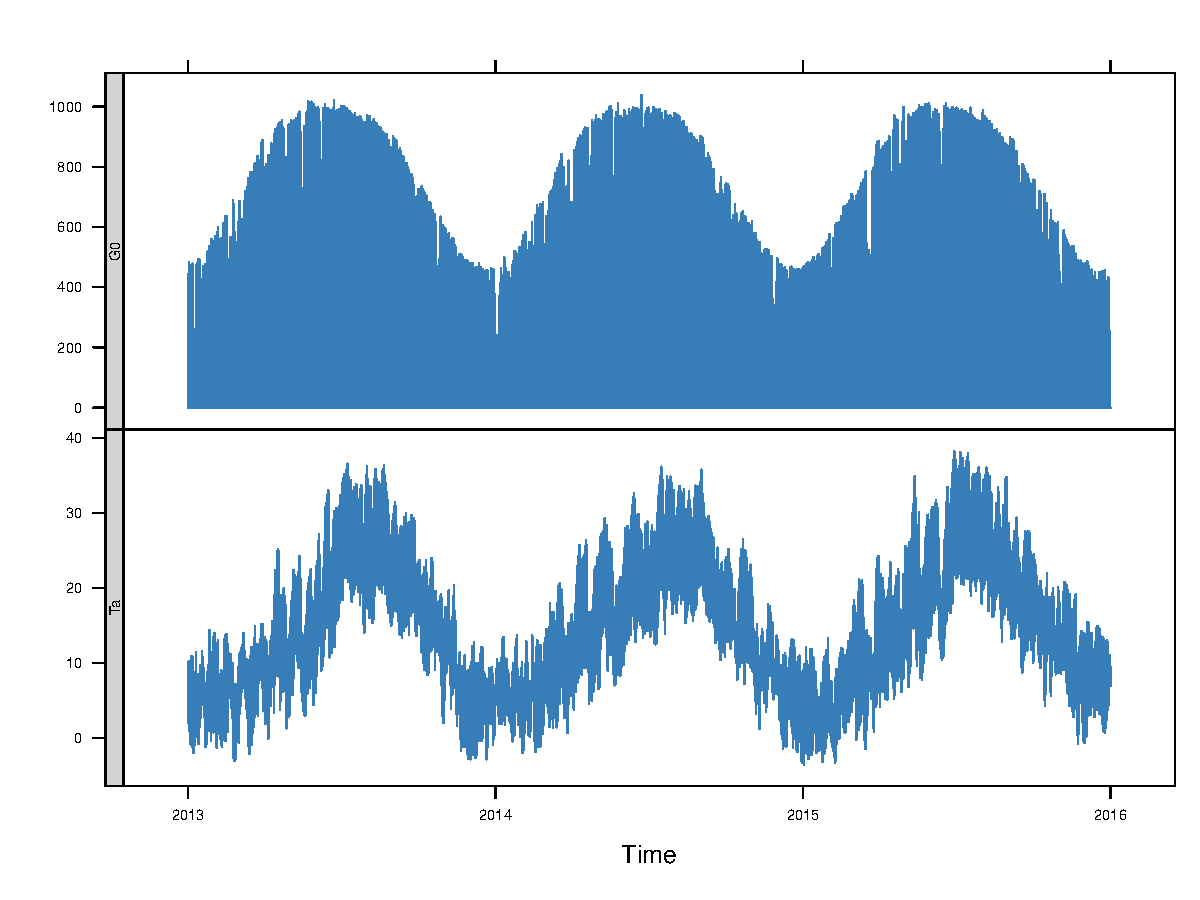
\includegraphics[width=\textwidth]{figuras/ejemplos1.pdf}
\end{center}

Una vez se tienen estos datos, se puede calcular la producción que van a tener los diferentes sistemas fotovoltaicos.

Para ello, se necesitan los parámetros de los diferentes sistemas. En la tabla \ref{tab:parametros-tecnicos-modulos-fotovoltaicos}, se pueden ver los distintos parámetros de los módulos fotovoltaicos.
\begin{center}
{\scriptsize }%
\begin{table}[]
{\scriptsize \caption{Parámetros técnicos de diferentes tipos de células solares.\label{tab:parametros-tecnicos-modulos-fotovoltaicos}}}
\centering{}{\scriptsize }\begin{tabular}{>{\centering}m{5cm} *{2}{>{\centering}m{2cm}}}
\toprule 
{\scriptsize \textbf{Parámetros Técnicos}} & {\scriptsize \textbf{mc-Si}} & {\scriptsize \textbf{pc-Si}}\tabularnewline
\midrule
{\scriptsize Potencia se salida (Wp)} & {\scriptsize 250} & {\scriptsize 220}\tabularnewline
{\scriptsize Voltaje en $P_{max}$ (Vmp)} & {\scriptsize 29.9} & {\scriptsize 29.0}\tabularnewline
{\scriptsize Corriente en $P_{max}$ (Imp)} & {\scriptsize 8.37} & {\scriptsize 7.59}\tabularnewline
{\scriptsize Voltaje en circuito abierto (Voc)} & {\scriptsize 37.1} & {\scriptsize 36.5}\tabularnewline
{\scriptsize Corriente en cortocircuito (Isc)} & {\scriptsize 8.76} & {\scriptsize 8.15}\tabularnewline
{\scriptsize Eficiencia del módulo (\%)} & {\scriptsize 15.5} & {\scriptsize 14.4} \tabularnewline
{\scriptsize $\alpha_{Isc}$ (\%/K)} & {\scriptsize 0.0043} & {\scriptsize 0.06} \tabularnewline
{\scriptsize $\beta_{Voc}$ (\%/K)} & {\scriptsize -0.338} & {\scriptsize -0.37}\tabularnewline
{\scriptsize $\gamma_{Pmpp}$ (\%/K)} & {\scriptsize -0.469} & {\scriptsize -0.45}\tabularnewline
{\scriptsize Temperatura NOC (ºC)} & {\scriptsize 43.7} & {\scriptsize 46}\tabularnewline
\bottomrule
\end{tabular}
\end{table}
\end{center}
Se almacena esta información en listas con la información de cada módulo.

\begin{lstlisting}[numbers=left,language=r,label= ,caption= ,captionpos=b]
## mc-Si
module1 <- list(Vocn = 37.1,
                Iscn = 8.76,
                Vmn = 29.9,
                Imn = 8.37,
                Ncs = 60,
                Ncp = 1,
                CoefVT = 0.00338,
                TONC = 43.7)
## pc-Si
module2 <- list(Vocn = 36.5,
                Iscn = 8.15,
                Vmn = 29,
                Imn = 7.59,
                Ncs = 60,
                Ncp = 1,
                CoefVT = 0.0037,
                TONC = 46)
\end{lstlisting}

Una vez se tiene la información de cada tipo de módulo, en la tabla \ref{tab:sistemas-fotovoltaicos} se pueden ver la información de la agrupación de cada sistema.
\begin{center}
{\footnotesize }%
\begin{table}
{\scriptsize \caption{Sistemas fotovoltaicos.\label{tab:sistemas-fotovoltaicos}}}
\centering{}{\scriptsize }\begin{tabular}{*{7}{>{\centering}m{1.85cm}}}
\toprule 
{\scriptsize \textbf{Sistema}} & {\scriptsize \textbf{Tecnología}} & {\scriptsize \textbf{Año de Fabricación}} & {\scriptsize \textbf{Módulos en Serie}} & {\scriptsize \textbf{Módulos en Paralelo}} & {\scriptsize \textbf{Potencia del Sistema STC ($Wp_{STC}$)}} & {\scriptsize \textbf{Tamaño ($m^2$)}}\tabularnewline
\midrule
{\scriptsize 1} & {\scriptsize mc-Si} & {\scriptsize 2012} & {\scriptsize 5} & {\scriptsize 1} & {\scriptsize 1250} & {\scriptsize 8}\tabularnewline
{\scriptsize 2} & {\scriptsize pc-Si} & {\scriptsize 2009} & {\scriptsize 5} & {\scriptsize 1} & {\scriptsize 1100} & {\scriptsize 8.2}\tabularnewline
\bottomrule
\end{tabular}
\end{table}
\end{center}
De la misma manera, se almacenará esta información en listas.

\begin{lstlisting}[numbers=left,language=r,label= ,caption= ,captionpos=b]
## mc-Si
generator1 <- list(Nms = 5, Nmp = 1)
## pc-Si
generator2 <- list(Nms = 5, Nmp = 1)
\end{lstlisting}

Una vez se tienen todos los parámetros del sistema fotovoltaico, se requieren los parámetros del inversor que tienen estos sistemas. Para facilitar el estudio, en el artículo explican que se usa el mismo inversor para todos los sistemas. Los parámetros de este se pueden ver en la tabla \ref{tab:caracteristicas-inversor}. 
\begin{center}
{\footnotesize }%
\begin{table}
{\scriptsize \caption{Carácteristicas del inversor.\label{tab:caracteristicas-inversor}}}
\centering{}{\scriptsize }\begin{tabular}{*{2}{>{\centering}m{5cm}}}
\toprule 
{\scriptsize \textbf{Inversor}} & {\scriptsize \textbf{SMA Sunny Boy-1200}} \tabularnewline
\midrule
{\scriptsize Potencia máxima DC} & {\scriptsize 1320 W} \tabularnewline
{\scriptsize Corriente máxima DC} & {\scriptsize 12.6 A} \tabularnewline
{\scriptsize Tensión máxima DC} & {\scriptsize 400 V} \tabularnewline
{\scriptsize Rango de tensión fotovoltaica (mpp)} & {\scriptsize 100-320 V} \tabularnewline
{\scriptsize Potencia máxima DC} & {\scriptsize 1320 W} \tabularnewline
{\scriptsize Potencia nominal de salida} & {\scriptsize 1200 W} \tabularnewline
{\scriptsize Maxima potencia aparente} & {\scriptsize 1200 VA} \tabularnewline
{\scriptsize Corriente máxima AC} & {\scriptsize 6.1 A}\tabularnewline
{\scriptsize Eficiencia} & {\scriptsize 92.1\%} \tabularnewline
\bottomrule
\end{tabular}
\end{table}
\end{center}

Se almacena esta información en otra lista:
\begin{lstlisting}[numbers=left,language=r,label= ,caption= ,captionpos=b]
inverter <- list(Ki = c(0.002, 0.005, 0.008),
                 Pinv = 1200,
                 Vmin = 100,
                 Vmax = 320,
                 Gumb = 20)
\end{lstlisting}

Una vez recopilada toda la información (la información que falta se deja sin añadir para que el propio paquete añada sus valores por defecto), se puede calcular la producción que tuvieron los sistemas:

\begin{lstlisting}[numbers=left,language=r,label= ,caption= ,captionpos=b]
prod1 <- prodGCPV(lat = 40.4, modeTrk = 'fixed', modeRad = 'bdI',
                  dataRad = etsidi_1315,
                  beta = 30, alfa = -19, 
                  module = module1, generator = generator1,
                  inverter = inverter)
prod2 <- prodGCPV(lat = 40.4, modeTrk = 'fixed', modeRad = 'bdI',
                  dataRad = etsidi_1315,
                  beta = 30, alfa = -19, 
                  module = module2, generator = generator2,
                  inverter = inverter)
compare(prod1, prod2)
\end{lstlisting}

\begin{lstlisting}[numbers=left,language=r,label= ,caption= ,captionpos=b]
show(as.zooY(prod1))
\end{lstlisting}

\begin{verbatim}
          Eac      Edc       Yf
2013 1681.077 1757.235 1343.449
2014 1698.613 1775.426 1357.463
2015 1749.536 1828.569 1398.158
\end{verbatim}


\begin{lstlisting}[numbers=left,language=r,label= ,caption= ,captionpos=b]
show(as.zooY(prod2))
\end{lstlisting}

\begin{verbatim}
          Eac      Edc       Yf
2013 1451.873 1517.779 1319.225
2014 1464.483 1530.833 1330.683
2015 1506.544 1574.704 1368.901
\end{verbatim}


\begin{center}
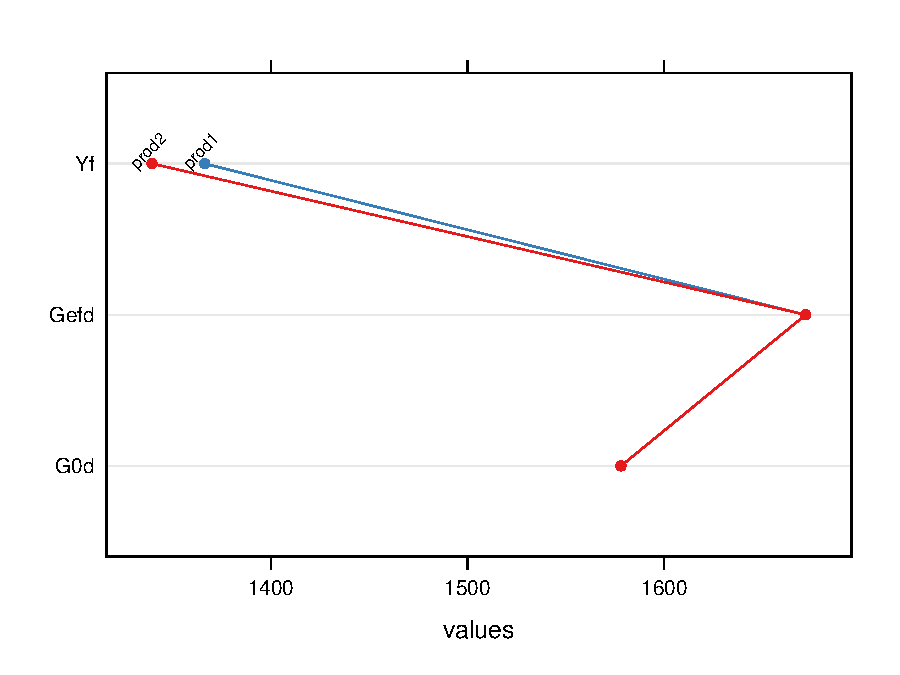
\includegraphics[width=.9\linewidth]{figuras/ejemplos2.pdf}
\end{center}
\section{\texttt{PVsyst}}
\label{sec:org3232024}
Con la herramienta \texttt{PVsyst}, se ha generado un año promedio de datos de irradiación en la localización y con estos datos se han obtenido dos informes (uno por cada sistema).

Por comodidad, en este documento se van a extraer solo unas tablas con los resultados principales. Sin embargo, los informes completos están disponibles en el \href{https://github.com/solarization/TFG\_Francisco\_Delgado\_Lopez}{github} del documento.

En las tablas \ref{tab:pvsyst1} y \ref{tab:pvsyst2} se tienen los resultados de la simulación de los sistemas.
\begin{center}
{\footnotesize }%
\begin{table}
{\scriptsize \caption{Energía media mensual estimada por \texttt{PVSyst} en $KWh$ del sistema 1.\label{tab:pvsyst1}}}
\centering{}{\scriptsize }\begin{tabular}{*{13}{>{\centering}m{0.75cm}}}
\toprule 
{\scriptsize \textbf{Ene}} & {\scriptsize \textbf{Feb}} & {\scriptsize \textbf{Mar}} & {\scriptsize \textbf{Abr}} & {\scriptsize \textbf{May}} & {\scriptsize \textbf{Jun}} & {\scriptsize \textbf{Jul}} & {\scriptsize \textbf{Ago}} & {\scriptsize \textbf{Sep}} & {\scriptsize \textbf{Oct}} & {\scriptsize \textbf{Nov}} & {\scriptsize \textbf{Dic}} & {\scriptsize \textbf{Total}}\tabularnewline
\midrule
{\scriptsize 3,7} & {\scriptsize 4,0} & {\scriptsize 5,6} & {\scriptsize 5,3} & {\scriptsize 6,7} & {\scriptsize 6,7} & {\scriptsize 7,9} & {\scriptsize 7,2} & {\scriptsize 6,4} & {\scriptsize 4,8} & {\scriptsize 3,5} & {\scriptsize 3,6} & {\scriptsize 1941,1} \tabularnewline
\bottomrule
\end{tabular}
\end{table}
\end{center}
\begin{center}
{\footnotesize }%
\begin{table}
{\scriptsize \caption{Energía media mensual estimada por \texttt{PVSyst} en $KWh$ del sistema 2.\label{tab:pvsyst2}}}
\centering{}{\scriptsize }\begin{tabular}{*{13}{>{\centering}m{0.75cm}}}
\toprule 
{\scriptsize \textbf{Ene}} & {\scriptsize \textbf{Feb}} & {\scriptsize \textbf{Mar}} & {\scriptsize \textbf{Abr}} & {\scriptsize \textbf{May}} & {\scriptsize \textbf{Jun}} & {\scriptsize \textbf{Jul}} & {\scriptsize \textbf{Ago}} & {\scriptsize \textbf{Sep}} & {\scriptsize \textbf{Oct}} & {\scriptsize \textbf{Nov}} & {\scriptsize \textbf{Dic}} & {\scriptsize \textbf{Total}}\tabularnewline
\midrule
{\scriptsize 4,3} & {\scriptsize 4,6} & {\scriptsize 6,4} & {\scriptsize 6,1} & {\scriptsize 7,3} & {\scriptsize 7,3} & {\scriptsize 8,3} & {\scriptsize 7,7} & {\scriptsize 6,9} & {\scriptsize 5,4} & {\scriptsize 4,1} & {\scriptsize 4,4} & {\scriptsize 2213,7} \tabularnewline
\bottomrule
\end{tabular}
\end{table}
\end{center}



\section{\texttt{solaR2}}
\label{sec:org7295038}
\label{sec:solaR2}
Con los datos obtenidos en la sección \ref{sec:solaR}, hacemos la misma operación pero con el paquete \texttt{solaR2}.
\begin{lstlisting}[numbers=left,language=r,label= ,caption= ,captionpos=b]
library(solaR2)
\end{lstlisting}

\begin{verbatim}
Cargando paquete requerido: data.table
data.table 1.15.4 using 6 threads (see ?getDTthreads).  Latest news: r-datatable.com
Cargando paquete requerido: lattice
Cargando paquete requerido: latticeExtra
Time Zone set to UTC.
\end{verbatim}


Para ello importamos de la misma manera los datos de radiación.
\begin{lstlisting}[numbers=left,language=r,label= ,caption= ,captionpos=b]
etsidi_1315 <- readBDi(file = 'TFG/data/PVGIS_1315.csv',
                       lat = 40.4, dates.col = 'Dates',
                       format = '%Y-%m-%d %H:%M:%S')
xyplot(etsidi_1315)
\end{lstlisting}

\begin{center}
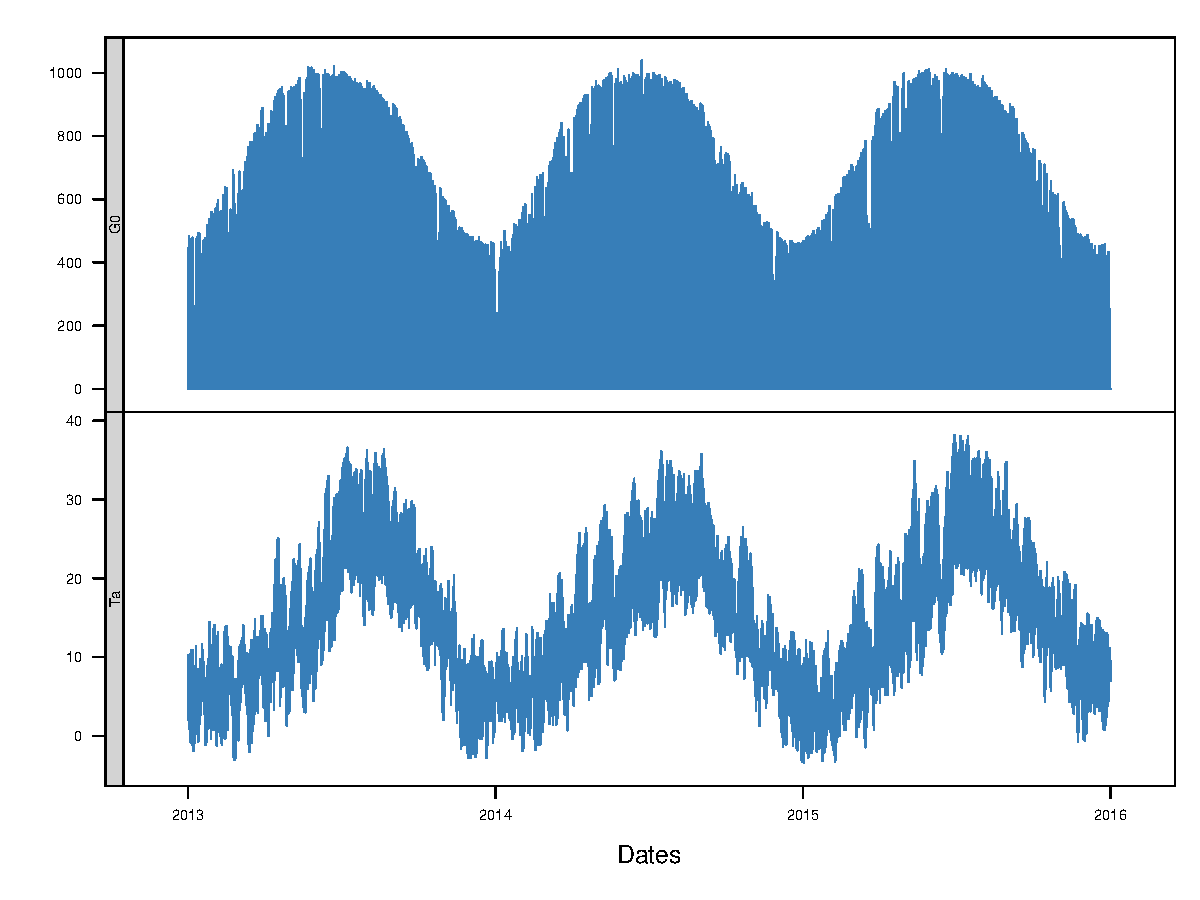
\includegraphics[width=\textwidth]{figuras/ejemplos3.pdf}
\end{center}
Con estos datos se procede al cálculo de la producción (los datos de los componentes del sistema son los mismos que los realizados en la sección \ref{sec:solaR}).
\begin{lstlisting}[numbers=left,language=r,label= ,caption= ,captionpos=b]
prod1 <- prodGCPV(lat = 40.4, modeTrk = 'fixed', modeRad = 'bdI',
                  dataRad = etsidi_1315,
                  beta = 30, alpha = -19, 
                  module = module1, generator = generator1,
                  inverter = inverter)
prod2 <- prodGCPV(lat = 40.4, modeTrk = 'fixed', modeRad = 'bdI',
                  dataRad = etsidi_1315,
                  beta = 30, alpha = -19, 
                  module = module2, generator = generator2,
                  inverter = inverter)
compare(prod1, prod2)
\end{lstlisting}

\begin{center}
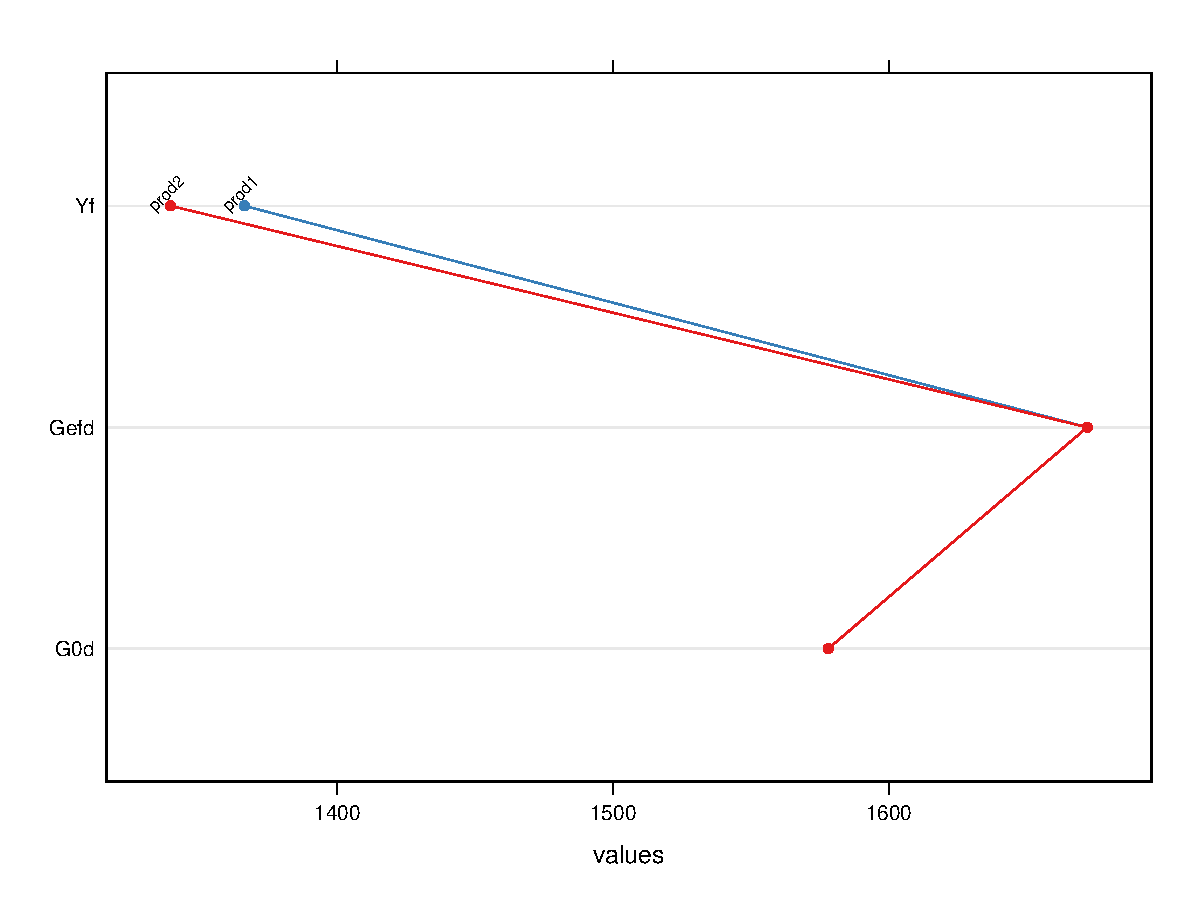
\includegraphics[width=\textwidth]{figuras/ejemplos4.pdf}
\end{center}
\begin{lstlisting}[numbers=left,language=r,label= ,caption= ,captionpos=b]
show(as.data.tableY(prod1))
\end{lstlisting}

\begin{verbatim}
   Dates      Eac      Edc       Yf
   <int>    <num>    <num>    <num>
1:  2013 1681.077 1757.235 1343.449
2:  2014 1698.613 1775.426 1357.463
3:  2015 1749.536 1828.569 1398.158
\end{verbatim}


\begin{lstlisting}[numbers=left,language=r,label= ,caption= ,captionpos=b]
show(as.data.tableY(prod2))
\end{lstlisting}

\begin{verbatim}
   Dates      Eac      Edc       Yf
   <int>    <num>    <num>    <num>
1:  2013 1451.873 1517.779 1319.225
2:  2014 1464.483 1530.833 1330.683
3:  2015 1506.544 1574.704 1368.901
\end{verbatim}

\section{Comparación y conclusiones}
\label{sec:org4b6368f}
\label{sec:comparacion-conclusiones}
Como se puede observar en las secciones anteriores, tanto el paquete \texttt{solaR} como el paquete \texttt{solaR2} ofrecen los mismos resultados, ya que toman las mismas referencias y estudios para realizar los cáculos. Sin embargo, el paquete \texttt{solaR2}, aparte de la corrección de algunos erores, presenta unas claras ventajas frente a su antecesor. Estas son:
\begin{itemize}
\item \textbf{Modularidad}: el paquete \texttt{solaR2} presenta muchas funciones que son capaces de realizar pequeñas operaciones, al contrario que \texttt{solaR}, que no permite esto.
\item \textbf{Eficiencia}: al estar basado en \texttt{data.table}, el paquete gana eficiencia en operaciones complejas. Para mostrar esto vamos a utilizar el paquete \texttt{microbenchmark}.
\begin{lstlisting}[numbers=left,language=r,label= ,caption= ,captionpos=b]
## Con el paquete solaR
library(microbenchmark)
## se recortan los datos a un solo año
etsidi_13 <- etsidi_1315[as.Date('2013-01-01'), as.Date('2013-12-31')]
prodGCPVcustom <- function(){  
  prod1 <- prodGCPV(lat = 40.4, modeTrk = 'fixed', modeRad = 'bdI',
                    dataRad = etsidi_13, beta = 30, alfa =-19,
                    module = module1, generator = generator1,
                    inverter = inverter)
}
microbenchmark(prodGCPVcustom(), times = 20)
\end{lstlisting}

\begin{verbatim}
Unit: milliseconds
             expr      min       lq     mean  median       uq      max neval
 prodGCPVcustom() 768.0936 781.2883 796.9569 790.474 814.2017 826.2135    20
\end{verbatim}


\begin{lstlisting}[numbers=left,language=r,label= ,caption= ,captionpos=b]
## Con el paquete solaR2
library(microbenchmark)
etsidi_13 <- etsidi_1315[as.Date('2013-01-01'), as.Date('2013-12-31')]
prodGCPVcustom <- function(){  
  prod1 <- prodGCPV(lat = 40.4, modeTrk = 'fixed', modeRad = 'bdI',
                    dataRad = etsidi_13, beta = 30, alpha =-19,
                    module = module1, generator = generator1,
                    inverter = inverter)
}
microbenchmark(prodGCPVcustom(), times = 20)
\end{lstlisting}

\begin{verbatim}
Unit: milliseconds
             expr      min       lq     mean   median       uq      max neval
 prodGCPVcustom() 522.1656 528.3605 535.2899 531.2649 537.8075 572.8096    20
\end{verbatim}
\end{itemize}
